%% ============================================================
%% 分片 14：原文第 5 节「Topological Field Theory In Two Dimensions」（原文 glshort.tex 起于第 3264 行）
%% 由 tools/harvmac2tex.py 从 arXiv 源码（hep-th/0604151v3）自动生成。
%% 只译英文散文；公式、编号、\label、\cite 一律不改。
%% ============================================================

\subsection{$S$-Duality Of the Hitchin Fibration}

\label{sec:sdualhitfib}

Our aim here and in section 第~\ref{sec:twodimint}~节\ is to show that
$S$-duality acts classically on the base of the Hitchin fibration
$\pi:\MH\to {\EUBB}$, while acting by $T$-duality on the fibers.

We recall that the base of the Hitchin fibration is a complex
vector space ${\EUBB}$. As described in section 第~\ref{sec:hitchfib}~节, the
linear functions on ${\EUBB}$ are the commuting Hamiltonians of
the integrable system $\MH$. They are of the form
% 式 (5.37)
\setcounter{equation}{36}
\begin{equation}\label{eq:utyr}
H_{{\cal P},\alpha}=\int_C\alpha {\cal P}(\varphi),
\end{equation}

where ${\cal P}$ is one of the fundamental homogeneous invariant
polynomials on the Lie algebra $\g$ of $G$. If ${\cal P}$  of
degree $n$, then $\alpha$ is an element of $H^1(C,K_C^{1-n})$. The
group ${\cal U}\cong \Bbb{C}^*$, which acts on $\varphi$ by
$\varphi\to\lambda\varphi$, acts as ${\cal P}\to \lambda^n{\cal
P}$.  This group action endows the holomorphic polynomial
functions on ${\EUBB}$ with the structure of a graded ring.

Roughly speaking, we want to show that $S$-duality preserves not
only the Hitchin fibration but also this graded ring of functions
on the base.  This statement is trivial for $T$ (which acts
trivially on everything in sight) so it is really a statement
about the duality transformation $S$.  $S$  maps $G$ to
$^L\negthinspace G$, and the claim is that it maps the sigma-model
of $\MH(G,C)$ to that of $\MH(^L\negthinspace G,C)$, mapping one
Hitchin fibration to the other, and preserving the grading.

 However, we need to explain exactly how to interpret
these notions quantum-mechanically. After compactifying the
topological gauge theory on $\Sigma\times C$, we pick a point
$z\in \Sigma$ and then, if ${\hat P}$ is any polynomial in the
$H_{{\cal P},\alpha}$'s, we evaluate ${\hat P}$ at $z$ to get a
local operator ${\EUO}_{\hat P}(z)$ in the effective
two-dimensional sigma-model on $\Sigma$. The operators of this
type, for any $z$, form a graded ring ${{\eurm R}}$; holomorphy in
$\varphi$ ensures that there are no singularities in products of
these operators.   The claim we wish to justify is that $S$
establishes an isomorphism between the graded rings ${{\eurm
R}}(G)$ and ${{\eurm R}}(^L\negthinspace G)$ for the two dual
groups. (There are no local operators analogous to the
${\EUO}_{\hat P}$'s that can be similarly used to measure the
fibers of the Hitchin fibration, so there is no analogous way to
show that $S$-duality acts classically on the fibers. It hardly
can, given its relation to mirror symmetry!)

The claim can be established directly by considering the
sigma-model with target $\MH$.  We simply note that in the
$B$-model of complex structure $I$, the ring we have just defined
is the same as the subring of ghost number zero (or cohomological
degree zero) of what is customarily called the chiral ring
\cite{ref78}. In general, in the $B$-model with target $X$, the
chiral ring is the bi-graded ring $H^q(X,\wedge^pTX)$ ($TX$ is the
tangent bundle of $X$). In particular, the subring of the chiral
ring with $p=q=0$  is just the ring of holomorphic functions on
$X$. But in complex structure $I$, a holomorphic function on $\MH$
must be constant on the fibers of the Hitchin fibration (which are
compact complex submanifolds) and hence must come from a
holomorphic function on the base.  So the holomorphic functions on
$\MH$, in complex structure $I$, are precisely the holomorphic
functions on ${\EUBB}$.  Now the duality transformation $S$
preserves the $B$-model in complex structure $I$, as we have
learned above, or more precisely it maps this $B$-model for
$\MH(G,C)$ to the corresponding model for $\MH(^L\negthinspace
G,C)$. So $S$ maps the chiral ring of $\MH(G,C)$ to that of
$\MH(^L\negthinspace G,C)$. Equivalently, the base ${\EUBB}$ of
the Hitchin fibration for $G$ maps to the analogous base
$^L\negthinspace{\EUBB}$ for $^L\negthinspace G$.  Moreover, $S$
commutes with the $R$-symmetry group ${\cal U}_1$ (the unitary
subgroup of ${\cal U}\cong \Bbb{C}^*$).  This plus holomorphy
ensures that the action of $S$ is compatible with the $\Bbb{C}^*$
action on the two sides.

What we have just seen is a typical example of exploiting the fact
that $\MH$ is a hyper-Kahler manifold.  We made the argument in
the $B$-model of complex structure $I$ even though we will apply
the results to the $B$-model in complex structure $J$ and the
$A$-model in complex structure $K$.

 One can argue the same result more explicitly
starting from four-dimensional gauge theory. The four-dimensional
argument gives more information; it will tell us precisely how the
duality acts on the base of the Hitchin fibration.

We begin with ${\EUN}=4$ super Yang-Mills theory
 on $\Bbb{R}^4$. For any positive integer $n$, let ${\EUD}_n$
(or $\EUD_n(G)$ if we wish to specify the gauge group) be the
space of local operators of the following form. An element of
${\EUD}_n$ is a $G$-invariant polynomial function ${\hat
Q}(\phi_0,\dots,\phi_5)$ in the $\phi_i$, homogeneous of degree
$n$, and moreover  constrained as follows: under $Spin(6)_{\cal
R}=SU(4)_{\cal R}$, $\hat Q$ transforms in the representation
${\rm Sym}_0^n{\bf 6}$ (the representation consisting of traceless
$n^{th}$ order polynomials in the ${\bf 6}$ or in other words the
irreducible representation whose highest weight is $n$ times the
highest weight of the ${\bf 6}$).

We interpret an element of ${\EUD}_n$ as a local operator that can
be evaluated at an arbitrary point $x\in \Bbb{R}^4$.  These
operators are precisely the  ``half-BPS'' operators of  dimension
$n$ in ${\EUN}=4$ super-Yang-Mills theory, that is, the operators
that are annihilated by one-half of the superconformal symmetries
that leave  fixed the point $x$.

Because the space ${\EUD}_n$ is defined by an intrinsic criterion
in terms of the action of supersymmetry, $S$-duality must
establish an isomorphism between $\EUD_n(G)$ and $\EUD_n(\LG)$. In
particular, if the Lie algebra of $G$ is selfdual (${\EUN}=4$
super Yang-Mills theory on $\RR^4$ depends only on the Lie algebra
of $G$), one could hope that $S$-duality acts trivially on
${\EUD}_n$. This is indeed true for simply-laced $G$, if the
scalars are normalized to have canonical kinetic energy, as can be
seen from string-theoretic derivations of $S$-duality. For $G_2$
and $F_4$, the duality transformation $S$ acts on ${\EUD}_n$ as a
nontrivial involution \cite{ref47}.

If the graded sum ${\EUD}=\oplus_n {\EUD}_n$ were  a graded ring
under operator products, we would use this ring to draw the
conclusions we want about the Hitchin fibration.  This actually is
not true, mainly because of the condition on how $\hat Q$
transforms under $Spin(6)_{\cal R}$.

We do, however, get a graded ring if we fix a Weyl chamber of
$Spin(6)_{\cal R}$  and restrict to those operators in ${\EUD}_n$
that transform as highest weight vectors. Indeed, consider the
subgroup $Spin(2)\times Spin(4)\subset Spin(6)_{{\cal R}}$, where,
in our construction of the twisted TQFT,  $Spin(2)$ rotates the
$\phi_2-\phi_3$ plane and $Spin(4)$ rotates the untwisted scalars.
(Thus, $Spin(2)$ is precisely the group ${\cal U}_1$ that acts by
phase rotations of $\varphi$.)   Then in the representation of
$Spin(6)$ spanned by the scalars $\phi_0,\dots,\phi_5$, the field
$\varphi$ can be interpreted as a highest weight vector, for some
choice of Weyl chamber. And the subspace ${\EUD}'_n\subset
{\EUD}_n$ of highest weight vectors consists of the
gauge-invariant polynomials $P(\varphi)$. Alternatively, these are
the $Spin(4)$-invariants with the largest possible eigenvalue of
$Spin(2)$.  Since $S$-duality commutes with $Spin(6)_{\cal R}$ and
hence with $Spin(2)\times Spin(4)$, these conditions are invariant
under $S$-duality.   Hence, $S$-duality maps ${\EUD}'_n$ to
itself.

Now ${\EUD}'=\oplus_{n\geq 0}{\EUD}'_n$ {\it does} form a graded
ring under operator products.  It is part of what is usually
called the chiral ring of the gauge theory (the operators
$P(\varphi)$ are chiral superfields with respect to one of the
supersymmetries, and their products are also chiral superfields).
The action of $S$ on ${\EUD}'$ preserves its structure as a graded
ring, since this structure is part of the operator product
expansion of the theory.

 The transformation of gauge-invariant polynomials in $\varphi$
under $S$-duality is, for dimensional and symmetry reasons, not
affected by twisting and compactification.  Moreover, a commuting
Hamiltonian $H_{{\cal P},\alpha}$ of degree $n$ in $\varphi$ is
obtained by integrating an element ${\cal P}(\varphi)\in\EUD'_n$
over $C$ (more exactly, over $z\times C\subset \Sigma\times C=M$,
for some point $z\in\Sigma$) with some weight $\alpha\in
H^1(C,K_C^{1-n})$. This process of integration over $C$ does not
affect the transformation under $S$-duality, so the action of
$S$-duality on the graded ring of holomorphic functions on the
base ${\EUBB}$ of the Hitchin fibration is simply determined by
the action on the four-dimensional graded ring $\EUD'$. In
particular, therefore, the transformation $S$ maps the base of the
Hitchin fibration of $G$ to the base of the Hitchin fibration for
$^L\negthinspace G$, intertwining between the two $\Bbb{C}^*$
actions.

\subsection{Two-Dimensional Interpretation Of $S$-Duality}

\label{sec:twodimint}

Now we can obtain a useful characterization of how the operation
$S$ acts on the sigma-model of target $\MH$.  Because the
$S$-transformation reduces essentially to mirror symmetry, we will
follow the insight of Strominger, Yau, and Zaslow \cite{ref79}: the key point
is to understand the action of $S$ on zerobranes. In this
analysis, and in much of our later discussion of branes, it will
suffice to consider branes in the effective two-dimensional
sigma-model of target $\MH$.  How to interpret these branes in the
underlying gauge theory is briefly discussed in section 第~\ref{sec:zapendix}~节\
and will be further described in \cite{ref26}. The picture we describe
has been argued \cite{ref18,ref19} previously and has been exploited
mathematically \cite{ref21}.

We start with a zerobrane ${\cal B}_p$ supported at a point $p\in
\MH(G,C)$. Like any brane, it corresponds to a boundary condition
in the sigma-model.  The specific meaning of a zerobrane supported
at $p$ is as follows: if this boundary condition is imposed on a
component $\gamma$ of the boundary of $\Sigma$ (in which case we
say that $\gamma$ is {\it labeled} by ${\cal B}_p$), this means
that the sigma-model map $\Phi:\Sigma\to\MH(G,C)$ maps $\gamma$ to
the point $p$.

A point is a complex submanifold in every complex structure. So a
zerobrane is what we will call a brane of type $(B,B,B)$; that is,
it is a $B$-brane in each of the three complex structures $I,J,K$.

\begin{figure}[htbp]
\centering
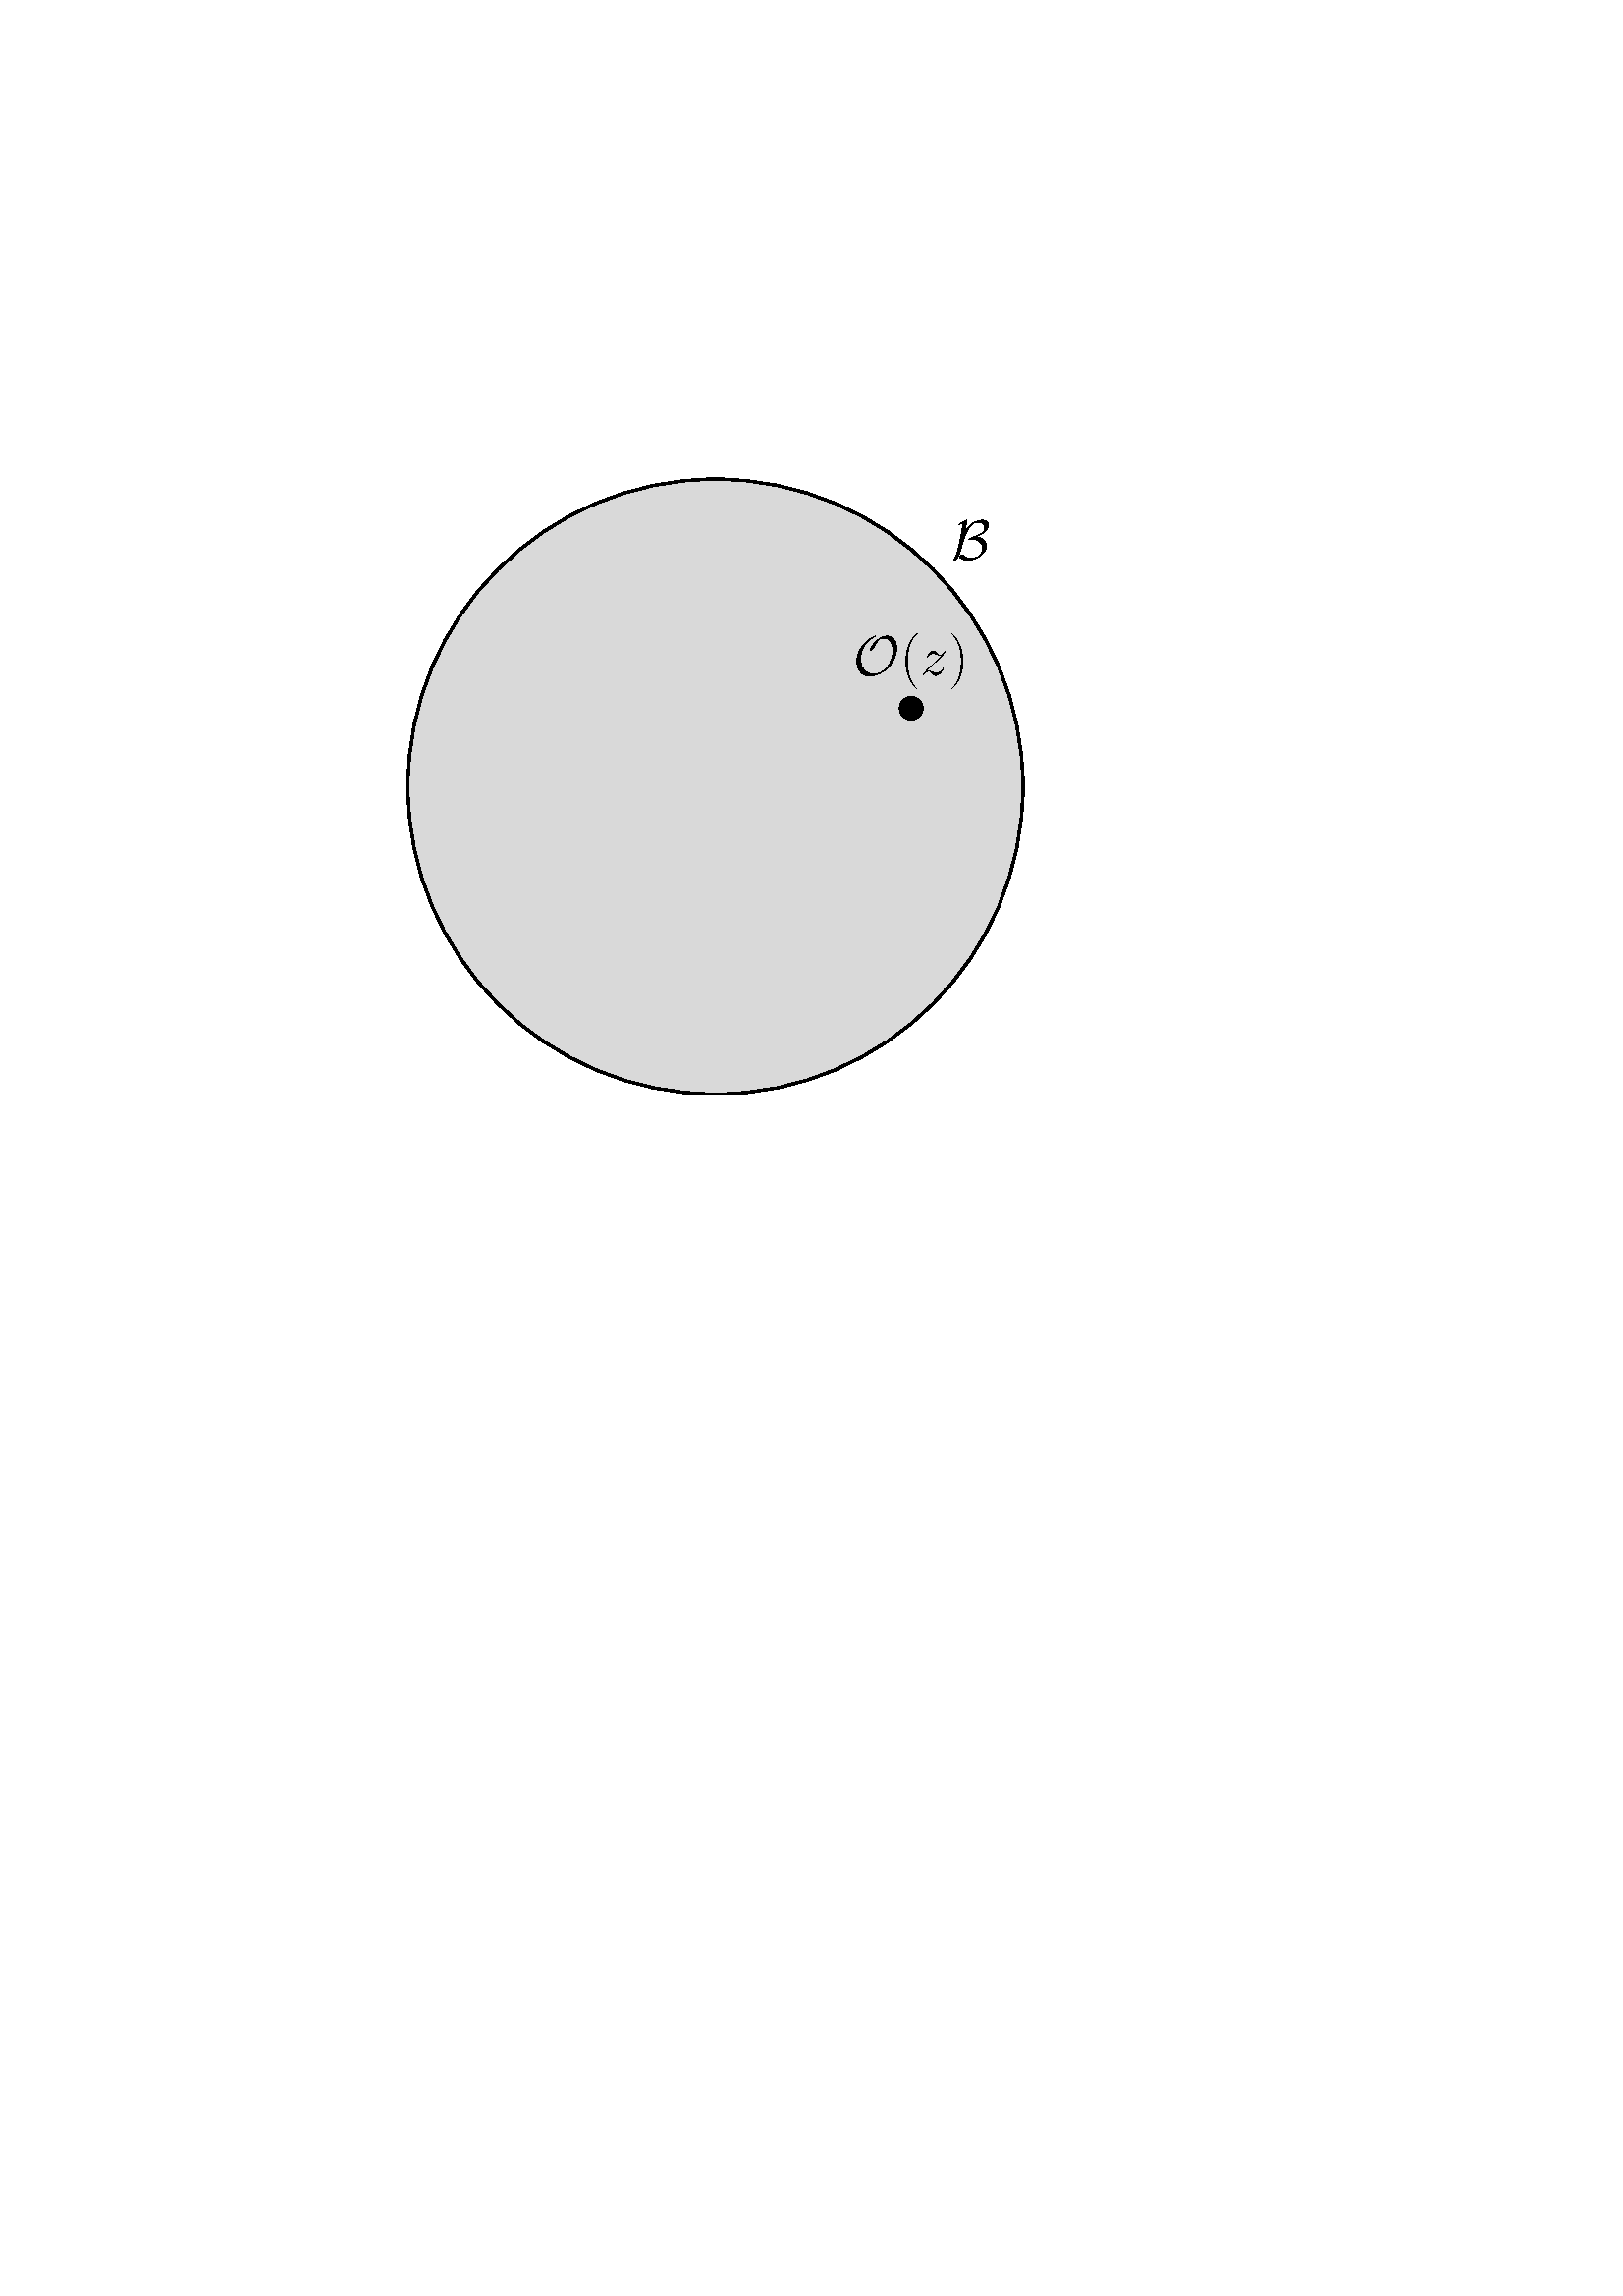
\includegraphics[width=0.75\linewidth]{figures/gla3-1.png}
\caption{ \medskip A local operator ${\EUO}(z)$ inserted at a point $z$ in the interior of a disc (shaded region) whose boundary is labeled by a brane ${\cal B}$. As $z$ approaches the boundary of the disc, ${\EUO}(z)$ may approach a complex constant. If this holds for suitable operators ${\EUO}_{H_\alpha}$, we say that ${\cal B}$ is supported on the fiber $\CMF$ of the Hitchin fibration.（原文 Fig.~3）}
\label{fig:trampo}
\end{figure}

Because the zerobrane is supported at a single point, it lies on a
single fiber $\CMF_p$ of the Hitchin  fibration.  This fiber is
characterized by equations $H_\alpha = h_\alpha$, where $H_\alpha$
are the commuting Hamiltonians and $h_\alpha$ are complex
constants.  Quantum mechanically, we say that a brane ${\cal B}$
is supported on a fiber ${\CMF}_p$
 if  the
operators ${\EUO}_{H_\alpha}(z)$, as $z$ approaches a boundary
labeled by the brane ${\cal B}$, approach the $c$-numbers
$h_\alpha$ (\trampo).  The brane ${\cal B}_p$ certainly has this
property.

Now we consider the duality operation $S$.  It replaces $G$ with
the Langlands dual group $^L\negthinspace G$, and so turns the
zerobrane ${\cal B}_p$ into a dual brane $\tilde{\cal B}_p$ in the
sigma-model whose target is $\MH(^L\negthinspace G,C)$. Looking
back at Table 2, we see that, since ${\cal B}_p$ is a brane of
type $(B,B,B)$, $\tilde {\cal B}_p$ will be a brane of type
$(B,A,A)$, that is, a $B$-brane in complex structure $I$ and an
$A$-brane in complex structures $J$ and $K$.

The transformation $S$ gives a map $\Xi:{\EUBB}\to
{}^L\negthinspace{\EUBB}$, where ${\EUBB}$ is the base of the
Hitchin fibration for $G$ and $^L\negthinspace{\EUBB}$ is its
analog for $^L\negthinspace G$.  Concretely, if a point $v\in
{\EUBB}$ is defined by equations $H_\alpha-h_\alpha=0$, and $S$
maps $H_{\alpha}$ to $^LH_{\alpha}$, then $\Xi(v)$ is defined by
equations $^LH_\alpha-h_\alpha=0$. As explained above, the map
$\Xi$ is the identity map for simply-laced $G$.

Applying $S$ to the situation of \trampo, we observe that if for a
brane ${\cal B}$, the operator ${\EUO}_{H_\alpha}(z)$ approaches
$h_\alpha$ as $z$ approaches the boundary, then for the dual brane
$\tilde {\cal B}$, the dual operator ${\EUO}_{\tilde H_\alpha}(z)$
likewise approaches $h_\alpha$ in the same limit.
 Hence, if ${\cal
B}$ is supported on a fiber ${\CMF}$ of the the Hitchin fibration
for $G$, then its $S$-dual is a brane $\tilde {\cal B}$ supported
on the corresponding fiber $\tilde {\CMF}=\Xi({\CMF})$ of the
Hitchin fibration for $^L\negthinspace G$.

Therefore, $\tilde{\cal B}_p$ is a brane of type $(B,A,A)$ that is
supported on a fiber $\tilde {\CMF}$ of the dual Hitchin
fibration. Let us focus on complex structures $J$ and $K$ in which
$\tilde{\cal B}_p$  is an $A$-brane.  In general, the support of
an $A$-brane in a space $X$ is at least middle-dimensional. The
most familiar $A$-branes are supported on middle-dimensional
Lagrangian submanifolds; there are also more exotic coisotropic
$A$-branes, with support above the middle dimension \cite{ref80}. But the middle dimension is the lower bound
on the dimension of the support of an $A$-brane.

However, an $A$-brane such as $\tilde {\cal B}_p$ that is
supported on the fiber $\tilde {\CMF}$ has support that is {\it at
most} middle-dimensional. To reconcile these constraints,
$\tilde{\cal B}_p$ must have support that is precisely $\tilde
{\CMF}$. Indeed, as explained in section 第~\ref{sec:hitchfib}~节, $\tilde
{\CMF}$ is holomorphic in complex structure $I$ and Lagrangian
with respect to symplectic structures $\omega_J$ and $\omega_K$.
So a brane wrapped on $\tilde {\CMF}$ and endowed with a flat
unitary Chan-Paton bundle ${\cal L}$ is indeed a brane of type
$(B,A,A)$.

Let us next compare the moduli on the two sides, restricting
ourselves to branes supported on ${\CMF}$ on one side or on
$\tilde {\CMF}$ on the other. With this restriction, the moduli
space of ${\cal B}_p$ is just a copy of ${\CMF}$: $p$ can be any
point in ${\CMF}$.

Meanwhile, the moduli of the dual brane $\tilde{\cal B}_p$ are a
complex torus  ${\EUJ}_{\tilde {\CMF}}$ that parametrizes flat
Chan-Paton bundles on $\tilde {\CMF}$ of rank 1. (The rank is 1,
as otherwise the moduli space of $\tilde{\cal B}_p$ would have
dimension greater than that of ${\cal B}_p$, and $S$-duality could
not hold.) ${\EUJ}_{\tilde {\CMF}}$ has the same dimension as
${\CMF}$ or $\tilde {\CMF}$. Clearly, $S$-duality establishes an
isomorphism between ${\CMF}$ and ${\EUJ}_{\tilde {\CMF}}$.

Of course, we could run this backwards.  A zerobrane in
$\MH(^L\negthinspace G,C)$ at a point in $\tilde {\CMF}$ is
similarly transformed by $S$ to a brane in $\MH(G,C)$ that is
wrapped on ${\CMF}$, and endowed with a flat unitary Chan-Paton
bundle. So $S$-duality likewise establishes an isomorphism between
$\tilde {\CMF}$ and ${\EUJ}_{\CMF}$, the moduli space of flat
Chan-Paton bundles on ${\CMF}$ of rank 1.

This picture is  SYZ duality between torus fibrations.  ${\CMF}$
parametrizes flat Chan-Paton bundles of rank one on $\tilde
{\CMF}$, and vice-versa.  Informally, we can describe this by
saying that the operation $S$ acts by a map
$\Xi:{\EUBB}\to{}^L\negthinspace{\EUBB}$ from the base of one
Hitchin fibration to the base of the dual fibration, together with
a $T$-duality on the corresponding torus fibers. This is the usual
SYZ picture of mirror symmetry, except that the map $\Xi$ is
usually assumed to be trivial.

That the corresponding fibers of the Hitchin fibrations for $G$
and $^L\negthinspace G$ are dual complex tori has been shown for
unitary groups by Hausel and Thaddeus \cite{ref21}. For the
exceptional Lie group $G_2$, this duality has been established
recently by Hitchin \cite{ref81}.  The
question has also been analyzed by Donagi and Pantev for any
semi-simple Lie group using an abstract approach to spectral
covers \cite{ref82}.  See also the work of Faltings
on $G$-bundles
\cite{ref83}.

A number of important subtleties about this duality have been
omitted in this explanation. Some questions involve the center and
fundamental group of $G$ and are discussed briefly in section
第~\ref{sec:centertop}~节. Other questions involve the role of a spin structure
on $C$ and will not be analyzed in this paper.  A discussion of
the role of spin structures and more detail on the role of the
center and fundamental group and the duality for unitary groups
will appear elsewhere \cite{ref26}.

\subsection{Branes On $\MH$}

\label{sec:mhbranes}

We have  met several interesting examples of branes on $\MH$ --
the zerobrane and the brane wrapped on a fiber.  We will encounter
others.  As in our initial examples, most of the important branes
will  have supersymmetric properties with respect to all three
complex structures $I$, $J$, and $K$, and this is very useful in
understanding their behavior.  The branes of most interest
preserve half the supersymmetry of the effective two-dimensional
sigma-model, which in turn has half the supersymmetry of the
underlying gauge theory.

Examples include $(B,B,B)$-branes, which are $B$-branes in each
complex structure $I,J,K$, as well as branes of type $(B,A,A)$,
$(A,B,A)$, and $(A,A,B)$, which are of $ B$-type in one complex
structure and of $ A$-type in the two others. We have already seen
examples of $S$ exchanging a brane of type $(B,B,B)$ with one of
type $(B,A,A)$. {}From Table 2, we further see that $S$ maps a
brane of type $(A,B,A)$ to another brane of the same type, and
likewise for a brane of type $(A,A,B)$.

It is not difficult to give  examples of branes of each of these
four types; they will be the important branes in our study of the
geometric Langlands program.   Of course, we can more generally
have a brane that is of $B$ type for any linear combination of the
complex structures $I,J$, and $K$, and of $A$-type for the two
orthogonal complex structures.\footnote{However, there are no branes
of type $(B,B,A)$.  A subvariety that is holomorphic in complex
structures $I$ and $J$ is automatically holomorphic in complex
structure $K$.  And there likewise are no branes of type
$(A,A,A)$.}

The zerobranes that we have already studied are the most obvious
branes of type $(B,B,B)$.   Other examples of $(B,B,B)$-branes are
space-filling branes, whose target is all of $\MH$, endowed with a
Chan-Paton vector bundle that is holomorphic in each of the three
complex structures. Bundles of that sort include the trivial
bundle as well as other examples whose role in the geometric
Langlands program will be discussed elsewhere \cite{ref26}.

A large class of examples  of $(B,A,A)$-branes is as follows. Let
$N$ be a complex submanifold of $\MH$ in complex structure $I$
which is a Lagrangian submanifold with respect to the holomorphic
symplectic structure $\Omega_I$, and hence with respect to
$\omega_J$ and $\omega_K$. Then  a brane supported on $N$ with
trivial Chan-Paton bundle is a $(B,A,A)$-brane. We have already
encountered one important example: $N$ might be a fiber of the
Hitchin fibration. For another example, we can take $N$ to be,
from the standpoint of complex structure $I$, the space of all
pairs $(E,\varphi)$  where $E$ is held fixed and $\varphi$ is
allowed to vary. {}From the point of view of gauge theory, this
means that $A_{\bar z}$ is held fixed up to a gauge
transformation, which ensures the vanishing of
$\Omega_I=(1/\pi)\int_C\,|d^2z|\,\Tr\,\delta
\phi_z\wedge\delta A_{\bar z}$.  Hence it gives us a brane of type
$(B,A,A)$.

Similarly, examples of $(A,B,A)$ and $(A,A,B)$-branes come from
complex Lagrangian manifolds with respect to the complex structure
$J$ or $K$. A simple example of a complex Lagrangian manifold in
complex structure $J$ is obtained simply by keeping ${\cal
A}_{\bar z}=A_{\bar z}+ i\phi_{\bar z}$ fixed and letting ${\cal
A}_z=A_z+i\phi_z$ vary. This gives us the family of all flat
$G_{{\Bbb{C}}}$ bundles that have a specified holomorphic
structure. Similarly, we get a complex Lagrangian manifold in
complex structure $K$ by specifying $A_{\bar z}-\phi_{\bar z}$ and
letting $A_z+\phi_z$ vary.  In section 第~\ref{sec:abranes}~节, we will construct
more sophisticated examples of branes of type $(A,B,A)$ or
$(A,A,B)$ as ``coisotropic branes.''
